% Instructor's Guide to Euclidean Geometry Notes
\documentclass{tufte-handout}

%\geometry{showframe}% for debugging purposes -- displays the margins

%%%% Packages to make things pretty
\usepackage{amsmath,amsthm}
\usepackage{booktabs}
\usepackage{graphicx}
\setkeys{Gin}{width=\linewidth,totalheight=\textheight,keepaspectratio}
\graphicspath{{graphics/}}
\usepackage{units}
\usepackage{fancyvrb}
\fvset{fontsize=\normalsize}
\usepackage{multicol}
\usepackage{pdfpages}
\usepackage{paralist}
\usepackage{fourier}

%%%% Theorem Environments
\theoremstyle{definition}
\swapnumbers
\newtheorem{problem}{Problem}[section]
\newtheorem{conjecture}[problem]{Conjecture}
\newtheorem*{definition}{Definition}
\newtheorem*{theorem}{Theorem}
\newtheorem{question}[problem]{Question}
\newtheorem{challenge}[problem]{Challenge}
\newtheorem*{postulate}{Postulate}

%%%%%


\title{Euclidean Geometry}
\author[Instructor's Manual]{Instructor's Manual}
\date{Spring 2016} 

\begin{document}

\maketitle

\begin{marginfigure}
    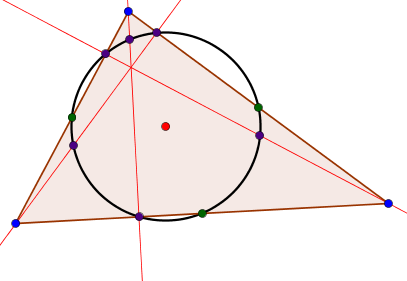
\includegraphics{NPC}
\end{marginfigure}


\setcounter{section}{0}
\setcounter{problem}{0}
\section{Instructor's Preface}

This opening section is a set of notes aimed at an instructor who wishes to use these notes for the first time.
I have deliberately aimed the discussion at someone who is \emph{new} to using inquiry-based methods in class.
More experienced instructors will know what to ignore and adapt things to their own style without much effort.
I hope newcomers to IBL will appreciate specific instructions about how I run a class from these notes.

Below the reader will find discussion of all of the major components of the course, and how I run the critically important first day.
Then I give some contextual notes for each item in the script, section-by-section.

\subsection{The Nature of this Course, and How it Came to Be}

idea of course: situational factors, big idea, main goals. idea of flexibility. definition wrangling, student-led conjecture work: expectation and permission\\

general non-sense goes here. philosophical advice. aims of the course. orientation stuff.  replace this later.\\

include Tim McNichol reference and idea

\subsection{Class Materials}

compass and straightedge, dynamic geometry software, Euclid from Green Lion Press, 
research notebook


\subsection{The First Class Meeting}

The importance of a good first meeting cannot be understated.
Students have to reach an understanding of how class will run and what is expected of them.
Also, at least one student has to have very visible success in front of the class.
It should also be possible to coax out a first student-made conjecture.
Here is how I run the first day:\\[.1in]

\begin{compactdesc}
\item[\textbf{Phase I}] I arrive early and put the first three definitions and Conjecture 1.1 on the board.
I reassure students that they don't need to copy this down, as I will hand it out to them later.
I also try to put them at ease with plenty of small talk about how I need to work out between semesters so that I can write so much.
This usually spills into the first minute or two of class.
When I am certain that the class is all present, I introduce myself briefly and ask them to try to prove the statement on the board with a partner.
I tell them that they should just use whatever they think they recall from high school geometry.\\[.1in]

\item[\textbf{Phase II}] Now I give the students time to work in pairs.
As they work, I go take the time to introduce myself to them and learn their names one pair at a time.
Along the way I have to take a couple of questions about mathematics, but mostly I am trying (1) to put faces to names on the roster and (2) to make myself more approachable.\\[.1in]

\item[\textbf{Phase III}] After about twenty five minutes, someone has an argument for at least part of Conjecture 1.1.
I call for volunteers, but if none materialize I call on a pair that I saw do something worthy.
I invite one student to come to the board to share their ideas.
After they get up, but before they start speaking, I interrupt and explain the basic ground rules to the class.\\[.1in]

We use only last names.
We are polite to a fault.
When in our seats, we ask questions rather than give arguments.
The presenter's job is to convince the class, but everyone else is trying to stay unconvinced as long as is reasonable.
We take ten to fifteen minutes to give the presentation and discuss it.\\[.1in]

Sometimes, the first presenter has a gap in their argument. 
In which case, it is important to do two things: (1) very clearly locate the error, and (2) find something of mathematical value in the presentation for which I can praise the student.
It is best if the class locates the error.
I try to do no more than ask if we are all in agreement.
Finding the praiseworthy aspect of a poor presentation is sometimes challenging, but you \emph{must} authentically praise an effort at the beginning of the course for something.
Then I bring up a second person.
When we have a completed argument, we thank the speakers with applause.\\[.1in]

\item[\textbf{Phase IV}] After the speaker, I explain that this is how we shall spend all of our class time.
I hand out the student's preface and the first section of problems (on the rhombus).
I explain that they should try to find proofs for the rest of Conjecture 1.1 and for the next few items before the next class.
We discuss that the point of the class is to gain power as a mathematician, and that means learning to find and defend our own arguments, so no outside sources are allowed.
I mention that collaboration is fine, but credit must be given.
At this point, we are usually just over time, so I let the class go with wishes for good luck.\\[.1in]
\end{compactdesc}

\subsection{Subsequent Meetings}

include note about usual progress. talk about "two students with different arguments for the same result."

\subsection{On the definition of a Polygon}

discussion about my loose defn of polygon.

\subsection{Student Made Conjectures \& the missing defns}

insight as to controlled conjecturing settings. basic ideas behind approach.


making definitions, why and how. 

include discussion of my very broad definition of a polygon.

euclid's definitions are sometimes crappy:
1. "point" really?
2. rhombus vs square vs rectangle




\subsection{Assessment}

daily work: specs approach. exams. assessment interviews.\\


I give one midterm examination and a final exam.
The midterm examination is in-class, and must be very focused.
I tend to pick four questions that get at important mathematical skills I might not have seen everyone perform, yet.
I usually only include one new argument, and it should be an adaptation of an argument that the students have seen more than once.
There simply is not time in a fifty minute exam to ask for several proofs of new statements.
An example is at the end of this guide.

The final examination is a week-long take-home.
I again ask four or five questions, each of which is new to the students.
There is usually one straightforward construction task.
I include this to be sure everyone has some measure of success on the exam.
I also include a conjecture that is a bi-conditional statement, one direction being false.
This is the challenging part of the exam: to notice the error, prove it is an error, and then repair the statement with the addition of a hypothesis.
If I have a question if a student deserves an A, quality work on this problem can change my mind.
An example exam is at the end of this guide.

\subsection{Advanced Students}

\subsection{Course Web Site \& The Class Blog}


\subsection{The Class Journal}

[[reference to paper about class journal in maa notes]]


\subsection{The Final Meeting}

\clearpage
\setcounter{section}{1}
\section{The Rhombus}

\begin{definition}
\label{defn:collinear}
We say that some set of points is \emph{collinear} when there exists a line passing through all of the given points.
\end{definition}

It is not always the case that my students have had instruction in basic set theory, so I try to stay away from the use of the word ``set'' as a formal thing. My students read the word ``set'' here as the common English word.


\begin{definition}\label{defn:quadrilateral}
A \emph{quadrilateral} is a figure consisting of four points, no three of which are collinear, in a given order and the four line segments joining points next to each other in the list.
Usually, we specify only the four points, so quadrilateral $ABCD$ consists of the points $A$, $B$, $C$ and $D$, called \emph{vertices} of the quadrilateral and the line segments $AB$, $BC$, $CD$ and $DA$, called the \emph{sides}.
\end{definition}

This definition is much closer to a clear and unambiguous technical definition. But it still has intended flaws. 
First, note that things are really stated twice, once without notation and then again with notation. 
In the version with notation, the importance of ordering the points is mentioned, but in the version with notation it is not. 
This will come up as a point of confusion at some time. 
In my experience, students will not notice the difference between the set of four points $\{A, B, C, D\}$ and the ordered sequence of four points $ABCD$ initially, but will later. 
When it happens, I use that as an opportunity for the students to clarify what they want and then state their own improved version with notation. 
This gives them some ownership of the mathematics.

Second, this definition allows for non-convex and even non-simple quadrilaterals. This is intentional. Having a more open definition simplifies some things and complicates others, and foreshadows the conversations about getting definitions sorted out that happens when we discuss the term ``polygon.''


\begin{definition}\label{defn:rhombus}
A \emph{rhombus} is a quadrilateral having all four sides mutually congruent.
\end{definition}

These first three are required to get through the first day of class! 


\begin{conjecture}
\label{conj:rhombus-angles}
Let $ABCD$ be a rhombus. Then angle $ABC$ is congruent to angle $ADC$. Similarly, angle $BAC$ is congruent to angle $BDC$.
\end{conjecture}

This conjecture is the object of the first day.
Note that the conjecture has two conclusions.
The first is true, but the second is false.
This is for two reasons:
(1) the figure relevant to the false statement encourages students to draw in the diagonal needed to find a simple proof of the first statement; and
(2) the point should be made early that not all conjectures in this course will be true.
Skepticism is important.

It is important that this theorem gets some sort of argument so that the process of presentation and discussion can be modeled before the students leave the first meeting.

Since this item is attempted during class on the first day, the resulting proof often lacks rigor in some key way. The most common way is that students do not quote triangle congruence theorems from Euclid properly, since they have not, yet, started to read it. This is easy enough for students to correct when they try to write the argument down with a copy of \emph{The Elements} at hand. 

Another common way is that students will draw both diagonals of the rhombus and give a proof that assumes these two diagonals meet. Of course, they do, but this will be unjustified, or justified by pointing to the diagram. 
This is a subtle error. If my students are making it and no 
one notices, I encourage them to introduce names for things and write up parts of their argument using those names.
That often helps students to see that a new point has been used without its existence being asserted. If students do not notice after that, I will take the otherwise unusual step of pointing it out. In any case, I help the students repair their work by adding a hypothesis to their theorem. It is important that the first class meeting has a theorem.\\

\begin{definition}\label{defn:diagonals}
Let $ABCD$ be a quadrilateral. The \emph{diagonals} of $ABCD$ are the segments $AC$ and $BD$.
\end{definition}

\begin{conjecture}
\label{conj:rhombus-diagonals}
The diagonals of a rhombus must cross.
\end{conjecture}

This item is very challenging.
Be careful not to let a weak student spin on it alone for too long, as it can become a trap that destroys their confidence.
Such a student should be encourage to work on other problems in parallel.

There are two natural arguments students make for this conjecture.
The first involves picking out a midpoint from one diagonal and proving that it lies on the other diagonal with the help of I.14.
This requires some creativity, and it doesn't always happen.

The second is a proof by contradiction that quickly splits up into many cases.
The second proof seems to be more common for my students, but they need help getting things organized.
This second proof also requires students to wrangle with the ideas behind ``the same side'' and ``opposite sides'' of a line.
If this is the route your class elects, don't be surprised if this problem is not solved until midterm time.
Setting up these missing terms from Euclid and proving a few very basic properties takes time and effort. But this kind of work, sorting out technical definitions for visually intuitive terms, is a big part of the work in these notes. This is just one of the concepts that Euclid does not give a satisfactory treatment, and the discomfort students feel about this is a good motivator for the importance of a clear and usable mathematical definition.


\begin{challenge}
\label{conj:rhombus-angles-redo}
If your argument for Conjecture \ref{conj:rhombus-angles} did not use Conjecture \ref{conj:rhombus-diagonals}, find a new argument that does.
Conversely, if your argument did use Conjecture \ref{conj:rhombus-diagonals}, find an argument that does not.
\end{challenge}

This is not strictly necessary, of course. 
Many semesters my students just ignore this item, but
it is included to make the point that many facts have more than one proof.
This encourages students to look for different avenues, or possibly to present a second proof of a result that a classmate has hit first.
I also use this as an opportunity to discuss the process of making extra hypotheses when stuck.

Note that the introductory paragraph in the student notes is phrased the way it is because I hand out the whole first section of tasks at the end of the first meeting, during which the students find a partial resolution to Conjecture \ref{conj:rhombus-angles}. If you use these notes differently, you will want to adjust this.


\begin{challenge}
\label{prob:rhombus-construct}
Given a segment $AB$, find a compass and straightedge construction of a rhombus $ABCD$.
Enumerate your steps and give a proof that the construction works.\footnote{A \emph{step} only counts if you draw something, like a segment or an arc of a circle.}
\end{challenge}

This is a straightforward construction task. When some variant of this has been presented successfully, I take control of class for a bit to lead several related conversations: 
(1) I discuss the change in tone from ancient Greek mathematics (if you can't construct it, it doesn't exist) to the modern constructive existence proof.
(2) I re-iterate what it means to enumerate steps (only things drawn with a compass or straightedge count), and how the presentation should have both a recipe for construction and a proof that this construction works.
(3) I lead a conjecture-making brainstorming session focused on the next task. 
This can all be accomplished in ten to fifteen minutes if done efficiently, but it is okay to allow more time for the important task of conjecture-making.

\begin{question}
\label{prob:rhombus-flexible}
How flexible or rigid is the construction solving the last problem?
Can one use the construction to create many non-congruent rhombi, or are there only a few options?
\end{question}

It is often the case that the first solution a class finds for Challenge \ref{prob:rhombus-construct} is just a special case.
This encourages a discussion which can lead to the general construction of the whole family of rhombi having a given side.
If students are encouraged, they will often ask good mathematical questions about the results here, and generate lots of official questions and conjectures for the class list. I have included this item in the official task list (rather than just waiting to bring it up in class) to make the point to students that they should start considering this kind of question. Having it here on the list also makes the class conversation after Challenge \ref{prob:rhombus-construct} more fruitful. I do not allow presentations for this item until the meeting after Challenge \ref{prob:rhombus-construct} has been presented successfully.

\begin{conjecture}
\label{conj:rhombus-is-parallelogram}
If $ABCD$ is a rhombus, then $ABCD$ is a parallelogram.
\end{conjecture}

Students very often come to class believing this is a property of rhombi, and they want to use it on the first day.
They get disappointed when it is pointed out this property is not part of the definition, so it is unavailable.
This conjecture lets them shore up their belief in the statement.

\begin{conjecture}
\label{conj:rhombus-diagonals-angle}
Let $ABCD$ be a rhombus. Suppose that the diagonals $AC$ and $BD$ meet at a point $X$.
The angle $AXB$ is a right angle.
\end{conjecture}

This result often gets proved very quickly, as it is a simple triangle congruence argument. I always stop things for a short discussion about how making an extra hypothesis can keep us from being stuck: we get to claim progress and we focus attention on what remains to be considered. I encourage them to work this way.

\clearpage
\setcounter{section}{2}
\setcounter{problem}{0}
\section{The Geometry of Kites}

This section of the tasks is designed to get students thinking about pushing their techniques, but being watchful for what is really true. Each of the statements here is an attempted generalization of a statement the students will have already considered for rhombi. 

\begin{definition}\label{defn:quad-sides-type}
Two sides of a quadrilateral are called \emph{adjacent} when they share a vertex and \emph{opposite} if they do not.
\end{definition}

\begin{definition}\label{defn:kite}
A \emph{kite} is a quadrilateral with two pairs of adjacent and congruent sides.
\end{definition}

Note that this definition would actually allow a figure with a set of three congruent sides. (My thanks to the referee who pointed it out.) No student in my course has, yet, noticed this. If it were to happen, I would make it another example of letting the students alter the official definition to suit their needs, sorting out the possible resolutions through experiment and conversation until we reach consensus as a class.

It is my experience that students will not initially consider a non-convex kite. My classes will show up the first meeting after these tasks have been distributed claiming to have finished all of them, but they will have errors from not having a broad enough imagination. I suppose the word ``kite'' 
evokes the idea of the traditional toy so strongly that they cannot see past it.
These tasks are partly designed to encourage the students to see that convexity is an issue.
Their arguments will often work just fine if the kites under consideration are ``like this,'' and not ``like that.'' In this way, we build the need for a new word and a clear definition of what counts as ``this'' and ``that.''
I avoid mentioning the word convex until after the students have expressed a need for the concept. In this setting, my students usually come up with a other language for particular examples (like a ``dart'' or a ``Star Trek kite''). We then set some class conjectures around sorting out the resulting mess.

\begin{conjecture}
\label{conj:kite-opp-angles}
Pairs of opposite angles in a kite are congruent.
\end{conjecture}

This is false. Rather, it is only partially true. A simple argument with congruent triangles will establish that one pair of opposite sides in a kite is always congruent. The other pair need not be. 

Students often have trouble stating their result precisely, and this should lead to a conversation about setting up notation and using it as a vehicle for clarity. After some attempts to state which pair of angles are congruent using natural language descriptions, students can appreciate the power and utility of naming the vertices of the kite and stating things in those terms. If notation doesn't magically appear, I usually ask the students to do a 2 minute writing exercise for a "good version" of the statement. Then I pair them up to critique for 2 minutes, and then we have a class discussion starting from their work. ("Please share an example where your partner's work is good.") If we move briskly, this is a well-spent 10 minutes.

The other conversation that comes up here is about how to prove something is false. Given the work on Conjecture 1.1, this is a chance to remind them about how counterexamples work: give an explicit construction of the example and prove it has the properties required. I do not always have this conversation in this exact spot, just to keep things moving.

\begin{conjecture}
\label{conj:kite-diagonals-cross}
The diagonals of a kite must cross.
\end{conjecture}

Again, this is false, but it requires the students to imagine a non-convex figure. The conversation about counterexamples should come up here if it has not already.

\begin{problem}
\label{prob:construct-kites}
Give a construction (with proof) of a kite.
How general is your construction?
\end{problem}

There is lots of room to work in this task. A student may or may not give the most general construction possible. I use this as an opportunity to have students ask questions and make conjectures about how flexible or free this construction is. It is not hard to get three or four interesting questions out of this. I add these to the task sequence immediately. Given the time to think about it in a brainstorming session, it is possible to get a conjecture along the lines of ``Given two segments and an angle, it is possible to construct a kite having the given segments as sides and the given angle between those sides." I have had classes state it as "Given a rhombus ABCD, it is possible to make choices in Ms. Y's construction to construct a rhombus congruent to ABCD."

\begin{conjecture}
\label{conj:kite-is-parallelogram}
If $ABCD$ is a kite, then it is a parallelogram.
\end{conjecture}

Again, this is false. Sometimes, students will approach this one in a non-constructive way, proving a statement like ``If ABCD is a kite and a parallelogram, then it is rhombus,'' taking it as a given that there exists a kite which is not a rhombus. Depending on the resolution of the 
previous items, they may already know that.


\begin{conjecture}
\label{conj:kite-diagonals-perpendicular}
If the diagonals of a kite meet, then they meet at a right angle.
\end{conjecture}

This leads to some good productive confusion. Expect students to have a disagreement about what is meant by the word ``diagonal.'' Some will think of it as a segment, and others will think of it as a line. I let the students have a conversation to sort it out. If they choose to change the definition to something different from that written in the tasks, I ask that they go back through their work and see what damage they may have wrought on previous work.

Many students will be confused by the need for the hypothesis, since it relates to convexity. In some classes, it is not until this point that students recognize that they need to consider such figures, and they have to go back and revise all of the work they have done on the other tasks in this section. 
There is a potential danger here: it would be a bad situation to have a week's worth of work somehow ``invalidated.'' Student morale would certainly suffer. But, as mentioned above, my students typically bring all of these tasks to one meeting and we find out things are not quite right before that day is out. 


\clearpage
\setcounter{section}{3}
\setcounter{problem}{0}
\section{The Geometry of Rectangles}

The most challenging aspect of this section for students is that they remember facts about rectangles, but often they are not sure which parts are part of the definition and which parts are theorems. We open with the definition as a reminder.

\begin{definition}\label{defn:rectangle}
A \emph{rectangle} is a quadrilateral which has all four interior angles that are right angles.
\end{definition}

\begin{conjecture}
\label{conj:rectangle-parallelogram}
Let $R$ be a rectangle. Then $R$ is a parallelogram.
\end{conjecture}

This item and the next are straightforward items, but they are the first times that students will be required to use results about parallel lines and right angles. A discussion of the parallel postulate might come up.

In any case, it is important to get the students to focus on using the definition as written, not as they vaguely recall.

\begin{conjecture}
\label{conj:rectangle-opp-sides}
Let $R$ be a rectangle. Then each pair of opposite sides of $R$ is a pair of congruent segments.
\end{conjecture}

This item can be derived as a simple consequence of the last and Euclid I.34. Students often just give their own proof independent of I.34.

I have had classes prove that this item is a consequence of the last item, and then also prove that the last item is a consequence of this one. It is then important to have a conversation about equivalent statements, and how we don't really know either of them, yet.

\begin{conjecture}
\label{conj:rectangle-diagonals}
The two diagonals of a rectangle are congruent and bisect each other.
\end{conjecture}

Beware! Students often just assume that the diagonals of a rectangle meet. If it seems to be sliding by the class, I will ask, "How do you know that point exists?" That will catch the presenter by surprise, so I often help them to modify their result by adding a hypothesis, and then we add an item to the student generated task sequence. Be sure to point out the similarity to Conjecture 1.2, though students will usually already see that.


\begin{conjecture}
\label{conj:opp-congruent-implies-rectangle}
Let $ABCD$ be a quadrilateral such that angles $\angle ABC$ and $\angle ADC$ are right angles.
If segments $AB$ and $CD$ are congruent, then $ABCD$ is a rectangle.
\end{conjecture}

This is incorrect, but in a sneaky way. As my definition of polygon allows for non-simple figures, it is possible to construct a counter example. Simply reflect half of a rectangle in one of its diagonals. Alternately, construct a non-isosceles right triangle and then reflect the legs in the perpendicular bisector of the hypotenuse.

Students often ``prove'' this result as written and get it past the class. When this happens, I try to find a way to make them realize it (without telling them) by asking pointed questions about how the assumptions in this item and the next one are different. 
It is also possible to address this when Thales' theorem in section 7 is proved.


\begin{conjecture}
\label{conj:opp-parallel-implies-rectangle}
Let $ABCD$ be a quadrilateral such that angles $\angle ABC$ and $\angle ADC$ are right angles.
If segments $AB$ and $CD$ are parallel, then $ABCD$ is a rectangle.
\end{conjecture}

This can trip students up as they try to give a proof by contradiction and use the parallel postulate at the same time. It helps to ask the students to work through the logic on this one extra slowly.

\begin{conjecture}
\label{conj:midline-theorem}
Let $ABC$ be a triangle, $D$ the midpoint of $AB$ and $E$ the midpoint of $AC$.
Then the line through $E$ and $D$, called a \emph{midline}, is parallel to the line through $B$ and $C$.
\end{conjecture}

This is challenging. Don't let a struggling student spin on it too long without help. This is sometimes called \emph{the midline theorem}. Students are sometimes tempted to use similar triangles to prove this result. This urge is natural, because generalizing the midline theorem to other values of the ratio $AD:AB$ is a way to build a theory of similar triangles.



\begin{conjecture}
\label{conj:Varignon}
Let $ABCD$ be a quadrilateral. The midpoints of the four sides are the vertices of a parallelogram.
\end{conjecture}

This pretty result is a simple corollary of the last item, if you draw diagonals of ABCD. Again, this can be an opportunity to show students that non-convex and non-simple figures exist. I usually ask students if they looked at this using GeoGebra, and then open up a GeoGebra sheet to show them how this looks when the input quadrilateral is dragged around. Students who have not considered it might ask "Does that count?" when they see those figures show up on the screen. This is an opportunity to start or continue the conversation.


\clearpage
\setcounter{section}{4}
\setcounter{problem}{0}
\section{Developing an Attitude of Skepticism}

The items in this short section sometimes don't get addressed completely. I find it acceptable to let them sit for a long time, because their mere existence is enough to make the point 
that students should not trust Euclid any more than they trust a classmate.

\begin{problem}\label{prob:Ball}
Read Professor Ball's argument and figure out what went wrong.
Recall that you can find it on the course web site under the "Class Journal" tab.
Pinpoint his error and present it to the class.
\marginnote[-20pt]{Prof. Ball uses a result he calls the hypotenuse-leg theorem, which states that if two right triangles have two pairs of corresponding sides congruent, and one of the pairs is the hypotenuses, then the triangles are congruent. For now, we grant that this theorem is true, and is not the source of Prof. Ball's error. We'll come back to address this theorem later when we study triangles in detail.}
\end{problem}

I post a copy of this nicely disguised fallacy on the my course web site as an example paper before the term begins. When students ask how to write their papers, I point to this as a simple guide for basic style. It is always my hope that some student reads this provocative argument and immediately objects. But I find that I have to explicitly ask my students to take up the task. 

\begin{problem}\label{prob:fix-I.7}
Figure out what is wrong with Euclid's Proposition I.7 and fix it.
\end{problem}

The trouble with Euclid I.7 is that only one case of many is considered. One can sort out which cases are missing and give each of them a similar short argument to settle the matter. The concept Euclid glides over is again a kind of ``betweenness,'' where points lie on either the same side or opposite sides of a line, just like Conjecture \ref{conj:rhombus-diagonals}. If it has not, yet, come up, this is an opportunity to set the students a class-made challenge about making good definitions for those concepts. 

\begin{problem}\label{prob:fix-I.4}
Figure out what the problem is with Euclid's Proposition I.4.
\end{problem}

This is the infamous ``Pons Asinorum.'' The trouble here is the use of superposition, and the lack of axiomatic support for that. I always lead a short clarifying discussion here about how this early proposition violates the spirit of the axiomatic method, and how modern writers often include I.4 as a postulate rather than as a theorem. (This applies to Hilbert's system, for example.)

\begin{problem}[Standing Problem]
As the semester progresses, we will have occasion to read over a hundred different arguments by Euclid, if any of the others we read have gaps, please consider giving a short presentation about it.
(Hint: there are several of these to be found.)
\end{problem}


\clearpage
\setcounter{section}{5}
\setcounter{problem}{0}
\section{Polygons}
Now it is time to extend our venue to \emph{polygons} with an arbitrary number of sides.

\begin{definition}\label{defn:n-gon}
Let $n$ be a natural number. An \emph{$n$-gon} is a figure consisting of $n$ points $A_1, A_2, \ldots, A_n$, prescribed in order and called \emph{vertices}, and the $n$ line segments, called \emph{sides}, $A_1A_2, A_2A_3, \ldots, A_{n-1}A_n, A_nA_1$.\\
A \emph{polygon} is an $n$-gon where $n$ has not been specified.
\marginnote[-20pt]{Note: Commonly used terminology includes the following: 3-gon = triangle, 4-gon = quadrilateral, 5-gon = pentagon, 6-gon = hexagon.}
\end{definition}

This definition is very open, and intentionally so. In fact, it introduces a conflict with the notion of a quadrilateral from earlier in the notes, in that a $4$-gon can have three collinear vertices. And there is still the problem of non-convex and non-simple figures. My students quickly become dissatisfied with the state of affairs and we end up having class conversations about what they believe to be a polygon and what they do not. I choose students to lead these conversations, and intentionally stay out of the way. It can take several days. I am careful to direct traffic by having the students pass the chalk around as the conversation moves, and I will jump up at some point and ask the students to make as many crazy examples as they can think of to show why the stated definition is not a good one. From this conversation should come several class-made conjectures and questions, now that we are really at the heart of the matter. Students will arrive at concepts like the following quite naturally:\begin{itemize}
\item What do we mean by a ``convex'' polygon?
\item What do we mean by a ``simple'' polygon?
\item What does it mean for two points to ``lie on one side'' of a
given line?
\item What does it mean for two points to ``lie on opposite sides'' of a given line?
\item What is a serviceable definition of the word polygon?
\item What does it mean to say that a point lies ``inside'' a given polygon?
\item What does it mean to say that a point lies on the ``inside'' of a given angle?
\end{itemize}
Be warned that this conversation could take several meetings. I ask the students to continue working on open problems while we are doing this, and I often give them a small challenge to prep for the next meeting to be sure the conversation continues. For example, ``Look at examples and decide for yourself if it is important to require that vertices of a polygon should be non-collinear. Be prepared to argue for your position and take a class vote next time.''

I allow the students to rewrite any of the definitions as long as they agree to it as a class, and then they have to abide by the consequences. At some point in this long conversation it will come up that students think I am withholding the ``correct'' definition from them. I take that opportunity to tell them that mathematics is a cooperative enterprise and our definitions are those that working mathematicians generally agree are the best for doing their job, and that has to be sorted out through conversation. 

\begin{problem}\label{prob:exterior-angle}
Suppose that $A,B,C$ are three consecutive vertices of a polygon. 
If at the vertex $B$ we extend one of the two sides through $B$ to a ray, then we create a new angle, called an \emph{exterior angle} to the polygon at $B$.\\
This construction has a choice in it. 
In principle, this could be a problem. 
Describe the problem, then state and prove a theorem that resolves the issue.
\end{problem}

This is intended to be an easy exercise to keep struggling students in the game. You might introduce the term ``vertical angles'' if the students do not do so on their own. Note that with the very generous definition of polygon above, the exterior angle of a non-convex figure could well point towards the inside. My students 
find this unsatisfactory and it helps spur them into making their own definitions.


\begin{conjecture}\label{conj:ext-angles-pentagon}
The exterior angles of a pentagon, one choice made at each vertex, add up to four right angles.
\end{conjecture}

This is true for convex pentagons, but false in general. Some semesters students will investigate enough with GeoGebra to 
prove interesting theorems about non-convex and non-simple figures. In any case, I always manage to get questions about those as class-made questions.

\begin{question}\label{question-induction}
What is the sum of the exterior angles of a hexagon? 
What about a general $n$-gon? 
Can you find a way to build on our understanding from small values of $n$, to general values of $n$?
\end{question}

This is the one opportunity to build up an inductive argument, if you are so inclined. Students will discover that a general polygon can be dissected into triangles, but probably will take that for granted. This is an opportunity to help students alter their hypothesis and make a meaty conjecture. 

\clearpage
\setcounter{section}{6}
\setcounter{problem}{0}
\section{Regular Figures, A Warm-up}

This section begins with some straightforward items. I reserve 
these for students who have not has as much success. I privately encourage students who are doing well in class to spend their energies on the rather more challenging class-made conjectures from the last section, and I privately encourage those who need a lift to spend a little more time on these tasks. 

\begin{definition}\label{defn:regular}
A polygon is said to be \emph{equilateral} if all of its sides are congruent, \emph{equiangular} if all of its angles are congruent, and \emph{regular} if it is both equilateral and equiangular.
\end{definition}

\begin{conjecture}\label{conj:equilateral-triangle}
An equilateral triangle is equiangular, hence regular.
\end{conjecture}

\begin{conjecture}\label{conj:regular-rhombus}
Let $ABCD$ be a rhombus. If angle $A$ is congruent to $B$, then $ABCD$ is regular.
\end{conjecture}

\begin{definition}[reminder]\label{defn:square}
A regular quadrilateral is called a \emph{square}.
\end{definition}


\begin{problem}\label{prob:equilateral-quad}
Does Conjecture \ref{conj:regular-rhombus} hold if we replace ``angle $B$'' by ``angle $C$''? State a result and prove it.
\end{problem}

The answer is ``No.'' This is an opportunity to reinforce how to write about counterexamples. 

\begin{conjecture}\label{conj:equilateral-pentagon}
Let $ABCDE$ be an equilateral pentagon. If angle $A$ is congruent to angle $B$, then $ABCDE$ is regular.
\end{conjecture}

This is false. When the class has progressed through these four items, I stop to point out how this is an example of 
systematic investigation of simple examples, structured in a natural way. This could be continued of course, but already pentagons show things are a bit more difficult. It is an opportunity to ask students to make some more conjectures of the same type as the above results. Sometimes my students state and prove theorems about equilateral pentagons with three angles congruent. 

\begin{conjecture}\label{conj:regular-pentagon-central-triangle}
Let $ABCDE$ be a regular pentagon. The triangle $ACD$ is isosceles.
\end{conjecture}

\begin{problem}\label{prob:reg-pentagon-angles}
Let $ABCDE$ be a regular pentagon. State the relationship between the angles $CAD$ and $ACD$ that shows how special the triangle is. Prove your observation.
\end{problem}

This is the challenging task in this set. The hardest part for my students is avoiding the use of measuring angles in degrees and instead stating their result as one about ratios of angles in the triangle $ACD$. (Angle $ACD$ is twice angle $CAD$.) Often, we find middle ground by getting a statement where angles are described as having some ratio to a right angle. (Angle $ACD$ is four fifths of a right angle.)

\begin{problem}\label{prob:reg-pentagon-types}
Find experimental evidence for the number of regular pentagons with a given side. (Try using five toothpicks!)\\[.1in]
\end{problem}

The results of this will depend upon what the class accepts as the definition of the word polygon. If they require polygons to have no self-intersections, there should be only the one. If they allow non-simple polygons then there will also be the five-pointed star.


\clearpage
\setcounter{section}{7}
\setcounter{problem}{0}
\section{Deeper Into Triangles}


\begin{problem}
\label{prob:triangle-inequality}
Show how to construct three segments which are not congruent to the sides of any triangle.
\end{problem}

Note that Euclid I.20 is a geometric statement of the triangle inequality. That makes this an easy task to complete. After this is successfully presented, I mention the triangle inequality and mention that it is a very important tool for modern mathematicians, especially in analysis. This is a conversation that can be expanded to touch upon more modern metric space geometry ideas if time permits, just to pique interest.

\begin{definition}
\label{defn:right-triangles}
A triangle is said to be \emph{right} if one of its angles is a right angle. 
The side opposite the right angle is called the \emph{hypotenuse}. 
The other sides are called \emph{legs}.
\end{definition}

\begin{conjecture}
\label{conj:RASS}
Let $ABC$ and $DEF$ be two right triangles, with the angles at $A$ and $D$ right angles. 
Suppose that $BC$ is congruent to $EF$ and $AB$ is congruent to $DE$. 
Then the triangles are congruent.
\marginnote{This is sometimes called the \emph{hypotenuse-leg} theorem.}
\end{conjecture}

Students are tempted to prove this using the Pythagorean Theorem (Euclid I.47). Note that this is not one of the propositions they have read so far. Instead, I require students to find another way. Ordinarily, students find an argument that relies on superimposing the two triangles. This relates to Problem \ref{prob:fix-I.4}. With some patient questioning, students can be coaxed to ``create a copy'' of one of the triangles in the place where they wanted to relocate it. This is a little tricky, and might take a few tries. 

\begin{conjecture}
\label{conj:ASS}
If we weaken the hypothesis of the previous conjecture so that the angles $A$ and $D$ are still congruent but no longer assumed to be right angles, and leave the other hypotheses intact, the conclusion still holds.
\end{conjecture}

This is false, but in an interesting way. Sometimes students will explore what they can say, and find there is only trouble when $A$ and $D$ are congruent obtuse angles, and even then there are only two possible triangles. This leads to a realization that the words acute and obtuse are really good for something geometric, and it allows for some open-ended inquiry for an enterprising student. At a time that feels appropriate, I will relate this to the difference between the Pythagorean Theorem and the Law of Cosines. One can say interesting things about how this relates to a quadratic equation having zero, one, or two solutions.


\begin{conjecture}
\label{conj:thales1}
If $AB$ is the diameter of a circle and $C$ lies on the circle, then angle $\angle ACB$ is a right angle.
\end{conjecture}

This is pretty easy, but it uses the common technique of drawing some key thing not originally in the figure. At this point I pause to point out how useful that is as a general technique in classical geometry, and suggest that they might try it on any outstanding open problems where they feel stuck. If appropriate, I then add, ``Hint. Hint. Conjecture \ref{conj:rhombus-diagonals}.''

\begin{conjecture}
\label{conj:thales2}
If $\angle ACB$ is a right angle, then $C$ lies on the circle with diameter $AB$.
\end{conjecture}

This direction is the harder of the two. I like a proof by contradiction best, because it ends up using Conjecture \ref{conj:thales1}. Note that there are two cases, but if you can handle one, the other comes along in a similar way.

Note that, together, Conjectures \ref{conj:thales1} and \ref{conj:thales2} yield this result:
\begin{theorem}[Thales' Theorem] 
Let $A, B, C$ be three points. 
The angle $\angle ACB$ is a right angle if and only if $C$ lies on the circle with diameter $AB$.
\end{theorem}

I always stop the class and have a short conversation about 
the idea of an ``if and only if`` statement. It is important to dispel the mystery of which part is which. I also share 
that some prefer the terms ``necessary and sufficient`` and discuss what those mean in context.

\clearpage
\setcounter{section}{8}
\setcounter{problem}{0}
\section{The Center of a Triangle}


\begin{conjecture}\label{conj:angle-bisectors-concurrent}
Let $ABC$ be a triangle, with rays $r$ and $s$ the angle bisectors at $A$ and $B$, respectively. Suppose that $r$ and $s$ meet at the point $I$ which lies inside the triangle. Draw lines $l$ and $m$ through $I$ that are perpendicular to $AC$ and $BC$ respectively. If $l$ meets $AC$ at point $X$ and $m$ meets $BC$ at $Y$, then triangle $IXC$ is congruent to triangle $IYC$.
\end{conjecture}



\begin{definition}\label{defn:concurrent}
Three segments (or lines or rays) are called \emph{concurrent} if they all pass through a common point.
\end{definition}

\begin{conjecture}\label{conj:incenter-concurrent}
The three angle bisectors of a triangle are concurrent.
\end{conjecture}

There are two subtle points here to discuss with the students. Following on from Conjecture \ref{conj:angle-bisectors-concurrent}, Conjecture \ref{conj:incenter-concurrent} feels like a quick corollary. But this relies on
the fact that two angle bisectors must actually meet so that we are in a situation to apply Conjecture \ref{conj:angle-bisectors-concurrent}. I prefer that the students notice it, of course, but I always make sure we discuss it and set an extra class-made task if the students have not included this step in their work. Also, the typical proof uses the idea that segment $IC$ has the property of an angle bisector at $C$, so it must be (part of) the angle bisector. That requires that the angle bisector of a given angle is \emph{unique}. Depending on time constraints, I might set this as a task for the students to prove, or I might just discuss it with them and sketch a proof briefly.

In either case, I always stop to point out the special nature of the configure and how we get an inscribed triangle whose center is a special point.

\begin{definition}\label{defn:incenter}
The point just discovered is called the \emph{incenter} of the triangle.
\end{definition}

\begin{conjecture}\label{conj:meeting-perp-bisectors}
Let $T$ be a triangle. For any pair of sides of $T$, the perpendicular bisectors of those sides meet. (That is, they are not parallel.)
\end{conjecture}

The typical argument here uses a proof by contradiction and the fifth postulate. It is a bit tricky to line everything up, so make the students go slowly.

\begin{conjecture}\label{conj:circumcenter}
The three perpendicular bisectors of any triangle are concurrent.
\end{conjecture}

Again, the expected argument relies upon a uniqueness claim in a subtle way.

\begin{definition}\label{defn:circumcenter}
The point where the three perpendicular bisectors of a triangle meet is called the \emph{circumcenter} of the triangle.
\end{definition}

Again, I pause to discuss how this shows a triangle has a circumscribed circle whose center is at an interesting point.

I often to ask students if they explored examples. It can be nice to use GeoGebra to see that the notions of a triangle being acute, right, or obtuse correspond to the location of the circumcenter relative to the triangle. If need be, I will open GeoGebra and make a quick demonstration.


If the mood strikes me, I might also point the students toward a web search for ``Triangle Center'' so that they may see the page at the url \url{http://faculty.evansville.edu/ck6/tcenters/}.


\clearpage
\setcounter{section}{9}
\setcounter{problem}{0}
\section{Circles}

It is finally time to have the students read more of Euclid, now in Book III. I ask them to read the parts that do not use any theory of area. 

\begin{conjecture}\label{conj:tangents-to-circle}
Let $AB$ and $AC$ be two tangent lines from a point $A$ outside a circle. Then $AB$ is congruent to $AC$.
\end{conjecture}

This is a simple consequence of the hypotenuse-leg theorem (Conjecture \ref{conj:RASS}). I reserve it for students who need a presentation.

\begin{definition}\label{defn:circles-perp}
We say that two circles \emph{meet at right angles} if the radii of the two circles to a point of intersection make a right angle.
\end{definition}

\begin{conjecture}\label{conj:perp-circles}
Let $\Gamma$ and $\Omega$ be two circles with centers $G$ and $O$, respectively. Suppose that these circles meet at two points $A$ and $B$. If $GAO$ is a right angle, then $GBO$ is a right angle.
\end{conjecture}

Again, this is a simple triangle congruence argument that I reserve for students who need a success. Depending on the time constraints of the semester, I may challenge the students to come up with a definition for the angle between two circles in general.

\begin{definition}\label{defn:cyclic-quad}
A quadrilateral $ABCD$ is said to be a \emph{cyclic quadrilateral} if there is a circle $\Gamma$ such that the four vertices $A,B,C$ and $D$ lie on $\Gamma$.
\end{definition}

\begin{conjecture}\label{conj:rect-cyclic}
A rectangle is always a cyclic quadrilateral.
\end{conjecture}

Depending on how well the students handled the material on rectangles this might be easy. If so, it is a good item for a student in need of a success.

\begin{conjecture}[Cyclic Quadrilateral Theorem]\label{conj:angles-cyclic-quad}
Let $A,B,C$ and $D$ be four points. The quadrilateral $ABCD$ is cyclic if and only if angle $DAC$ is congruent to $DBC$.
\end{conjecture}

This bi-conditional statement often gets proved in pieces, with different parts being proved by different students, since it naturally involves two theorems. If the students have continued on with my rather generous definition of polygon, this is false as stated. A non-simple cyclic quadrilateral has slightly different behavior. But that is interesting, too. I urge the students to set their own questions and conjectures and we add them to the class list.


\begin{conjecture}\label{conj:tangent-to-two-circles}
Let two circles be tangent at a point $A$. If two lines are drawn through $A$ meeting one circle at further points $B$ and $C$ and meeting the other circle at points $D$ and $E$, then $BC$ is parallel to $DE$.
\end{conjecture}

This is an application of Euclid III.32. If the students do not find III.32, this might take a while to resolve.

\clearpage
\setcounter{section}{10}
\setcounter{problem}{0}
\section{Circles, Coming 'Round Again}

This entire section consists of more challenging results about circles that may be omitted if you are running out of time and want to get to other material. In an ideal situation, one can encourage students who need more challenging material to work on these while their classmates
work on the last section.

\begin{conjecture}
Let $\Gamma$ be a circle with center $O$. Let $X$ be a point in the interior of the circle, and suppose that two lines $\ell$ and $m$ intersect at $X$ so that $\ell$ meets $\Gamma$ at points $A$ and $A'$ and $m$ meets $\Gamma$ at $B$ and $B'$.
Then twice angle $AXB$ is congruent to angle $AOB$ and angle $A'OB'$ taken together.
\end{conjecture}

\begin{question}
Consider the situation from the last conjecture, but instead assume that $X$ lies outside $\Gamma$. What happens here? Formulate a conjecture.
\end{question}


\begin{conjecture}
If two chords of a circle subtend different acute angles at points of a circle, then the smaller angle belongs to the shorter chord.
\end{conjecture}

\begin{conjecture}
If a triangle has two different angles, then the smaller angle has the longer angle bisector (measured from the vertex to the opposite side).
\end{conjecture}

\begin{conjecture}[Steiner-Lehmus]
If a triangle has two angle bisectors which are congruent (measured from the vertex to the opposite side), then the triangle is isosceles.
\end{conjecture}

\begin{conjecture}
Let $BC$ be a chord of circle $\mathcal{C}$, let $\widearc{BC}$ be the arc of $\mathcal{C}$ which is bounded by $B$ and $C$ and does not contain the center of $\mathcal{C}$.
Let $M$ be the midpoint of $\widearc{BC}$.
For a point $A$ on the arc $\widearc{BC}$, show that as $A$ moves along the arc from $B$ to $M$, the sums $AB+AC$ increase.
\end{conjecture}


The next theorem is very pretty, and is commonly attributed to Archimedes.

\begin{conjecture}[Archimedes' Theorem of the Broken Chord] Let $AB$ and $BC$ be two chords of a circle $\mathcal{C}$, where $BC$ is greater than $AB$.
(Such a configuration is sometimes called a ``broken chord.'')
Let $M$ be the midpoint of arc ${ABC}$ and $F$ the foot of the perpendicular from $M$ to chord $BC$.
Then $F$ is the midpoint of the broken chord, that is, $AB$ and $BF$ taken together are congruent to $FC$.
\end{conjecture}



\clearpage
\section{Appendix: Supplementary Documents}

syllabus, student conjectures list from fall 2015, exams from fall 2015, reflective writing prompts, specs/standards docs, writing info docs, conclusion handout

\end{document}


